\section{Datacenter}
Il \textbf{Datacenter} è una struttura composta da calcolatori che comunicano in rete, che aziende ed altre organizzazioni usano per organizzare, processare, memorizzare e disseminare enormi ammontare di dati. Essi rappresentano il cuore del business di un'organizzazione ed è necessario che soddisfino caratteristiche come scalabilità, sicurezza ed affidabilità oltre a possedere tutta l'attrezzatura necessaria come ad esempio la ventilazione, gruppi di continuità, sistemi di raffreddamento e naturalmente lo spazio necessario per installare il tutto. L'infrastruttura di un datacenter è cambiata molto durante gli anni e possiamo classificarla in tre categorie: 
\begin{description}
  \item[Infrastruttura Legacy:] In questa disposizione l'hardware è formato da tante commodity machines ma con l'obbligo di dover gestire ogni macchina separatamente ovvero si è costretti a dover installare su ogni macchina il sistema operativo, i programmi e le librerie necessarie. Da un primo impatto si può facilmente capire che con un numero molto grande di macchine la cosa risulta praticamente ingestibile e infatti questo modello è stato subito sostituito a favore delle architetture convergenti.
  \item[Infrastruttura Convergente:] In questa disposizione l'hardware è formato da enormi centri di calcolo che a differenza della struttura legacy sono gestiti tramite l'ausilio di un hypervisor quindi favorendo la gestione delle macchine ma con dei limiti dal punto di vista delle prestazioni in quanto la comunicazione con i dispositivi di memorizzazione avviene tramite una SAN\footnote{Storage Area Network} che rappresenta un collo di bottiglia nell'accedere e scrivere ai dati su disco.
  \item[Infrastruttura Iperconvergente:] Rappresenta la soluzione moderna per offrire un centro di calcolo performante. Questa architettura riprende il meglio delle due precedenti in quanto fa uso di commodity hardware, che costa poco, utilizza un hypervisor per gestire il datacenter ma la memorizzazione dei dati non avviene tramite una SAN. Quello che accade è che ogni rack possiede un insieme di piani che permette di aggiungere una motherboard formata da cpu, ram, e disco in modo che i dati delle singole motherboard possono accedere in maniera locale ai propri dischi aumentando le prestazioni e inoltre favorisce la scalabilità in quanto basta aggiungere al rack nuove motherboard quando è strettamente necessario.  
\end{description}
\begin{figure}[ht]
  \begin{center}
    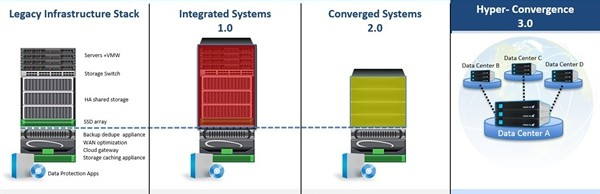
\includegraphics[width=\linewidth]{hyperconvergence.jpg}
    \caption{Le tre architetture}
    \label{hyp}
  \end{center}
\end{figure}
\section{Hypervisor}
%TODO parlare in dettaglio dell vmm aggiungere citazione DISCO(seminario antonio Tino)
Ogni commodity hardware che forma il moderno datacenter non si limita all'esecuzione di un unico sistema operativo in quanto questo rappresenterebbe uno spreco di risorse di memoria e di CPU che possono essede dedicate per eseguire altro calcolo. La virtualizzazione è stata la tecnologia fondamentale che ha permesso alle architetture dei datacenter di evolversi da legacy a convergenti. L'hypervisor rappresenta il componente software o hardware necessario per ottenere virtualizzazione e quando Bugnon nel 97 presentò Disco\cite{bugnon97} e il VMM (sta per virtual machine monitor ed è un sinonimo di hypervisor) nessuno avrebbe mai pensato che la sua intuizione lo avrebbe portato al successo fondando VMware.
\section{Gestione dello storage}
Essendo che un datacenter deve processare e memorizzare ordini di petabyte, quindi che non entrano in un disco commerciale, è stato necessario trovare delle soluzioni adeguate. La storia ci insegna che inizialmente i dati venivano memorizzati in enormi dischi rigidi (ricordiamo ad esempio SLED di IBM) che non solo costavano tantissimo ma occupavano tanto spazio con altezze che arrivavano addirittura a 14 pollici. La soluzione è arrivata nel 1988 grazie a Patterson e alla sua architettura \textbf{RAID} che ha evidenziato con i suoi esperimenti\cite{patterson88} che è possibile ottenere, mettendo insieme un array di dischi economici con appositi controller, più memoria, migliori prestazioni e tolleranza ai guasti.
\subsection{RAID}
L'acronimo sta per \textit{Redundant Array of Inexpensive Disks} e rappresenta l'innovazione che ha permesso di raggruppare diversi dischi dando la sensazione al sistema che possano essere utilizzati come se fossero un unico volume. L'implementazione del RAID può essere effettuata o hardware o software dove nel primo caso si usano controller hardware fatti a hoc molto costosi (più di tutti i dischi messi assieme), nel secondo caso il tutto viene gestito dal sistema operativo con un normale controller (che può essere SATA, ATI, SCSI, in fibra). Il tipo di array viene identificato dal livello RAID che determina il numero di dischi minimo necessario per poter essere configurato. La caratteristica fondamentale di questa tecnologia è quella della ridondanza che permette di individuare e correggere errori ed è ottenuta con differenti tecniche che variano a seconda del livello di RAID utilizzato:
\begin{description} 
  \item[RAID 0:]Questo livello non possiede ridondanza e utilizza lo \textbf{striping} (unità minima in cui viene diviso ogni file per la scrittura) per distribuire i file nei dischi facendo si che le letture e scritture avvengano in parallelo. Ha come svantaggio naturalmente la perdita totale dei dati in caso di rottura del disco.
  \item[RAID 1:]Questo livello dedica fa sì che alcuni dischi vengano usati come copia per i dati in modo da intervenire in caso di guasto. Dal punto di vista delle prestazioni siamo pari a quelle di un singolo disco ma è presente la fault tolerance.
  \item[RAID 2:] Questo livello presenta delle caratteristiche simile al livello 1 ma con l'aggiunta di codici di correzione ECC dei dati. Questa configurazione è caduta in disuso a causa del fatto che ora i dischi attuali implementano di suo questa tipologia di correzione.
  \item[RAID 3:] Questo livello utilizza sia lo striping che il controllo della parità. Lo striping viene applicato a livello di segmenti e la parità mantiene le informazioni necessarie per poter recuperare i dati persi. In questo livello le scritture peggiorano poichè ad ogni scrittura si affianca il calcolo della parità e inolre la scrittura di essa avviene in un unico disco causando un collo di bottiglia sulle prestazioni totali.
  \item[RAID 4:] Questo livello utilizza le stesse funzionalità del livello 3 con la differenza che lo striping non viene effettuato con i segmenti ma a livello di blocchi.
  \item[RAID 5:] Questo livello utilizza le stesse funzionalità del livello 4 ma con la differenza che in questa configrazione non esiste un unico disco per la scrittura della parità ma su tutti vengono scritti dati o calcolo di parità (da notare che la parità non viene scritta sullo stesso disco dei dati). RAID 5 ha delle buone prestazioni che tendono a migliorare con l'aumento dei dischi installati.
  \item[RAID 6:] Questo livello ha le medesime caratteristiche del livello 5 con la differenza che effettua un doppio calcolo della parità (tramite codici di Solomon). Le prestazioni sono le medesime di RAID 5 con la presenza di una ridondanza aggiuntiva dei dati di controllo a causa della parità.
  \item[RAID Annidati:] Sono combinazioni di configurazioni di RAID permettendo così di accorpare le caratteristiche dei livelli. Le due combinazioni più diffuse sono la 01 e la 10. La prima prende due configurazioni RAID 0 e le combina in un RAID 1 e questo comporta che ogni gruppo di dischi conterrà la copia speculare dell'altro gruppo. Il secondo prende gruppi di dischi in RAID 1 e si combinano in RAID 0 permettendo così di vedere il tutto come se fosse un unico disco e inoltre permette la tolleranza del guasto di sue dischi.
\end{description}
\subsection{Software Defined Storage}
%TODO argomentare meglio di cosa si tratta e spiegare meglio Ceph
Ceph è una piattaforma di storage distribuito creata da Red Hat recentemente (2016) e rappresenta quella che potrebbe essere in futuro una valida alternativa a RAID per gestire la memorizzazione dei dati. Questa piattaforma fornisce intefacce di storage di diverse tipologie (a oggetti, a file) quindi permettendo una grande flessibilità ma soprattutto riesce a scalare nell'ordine degli exabyte. La replicazione dei dati avviene al livello software rendendo così Ceph una piattafroma indipendente dall'hardware. La ragione del suo successo risiede nel fatto che sia possibile accedere ai dati in maniera completamente trasparente e diversificata permettendo di adattarsi alle esigenze delle organizzazioni. Un'altra caratteristica a fvore è che un sistema Ceph può essere costruito con commodity hardware riducendo di molto i costi a discapito di un controller RAID hardware.
\section{Sistema Operativo}
%TODO Aggiungere dettagli. Storia dei sistemi operativi SPIN, TORNADO.
Qui si parla dell'importanza del sistema operativo in ambiente distribuito.
\subsection{Kernel}
%TODO aggiungere microkernel, monolitico ed exokernel
Qui si parla delle varie architetture kernel.
\section{File System} 
In un data-center è indispensabile avere un filesystem che sia trasparente e che nasconda all'utente che usufruisce del cluster l'effettiva locazione dei file sui dischi. L'informatica ha conosciuto due diverse filosofie di implementazioni di filesystem su reti: I primi tentativi concreti sono stati ottenuti con l'introduzione del protocollo \textbf{SMB} (Server Message Block) ed è ancora tuttora utilizzato da Windows e da Linux (Samba), successivamente negli verso la metà degli anni 80 alla Carnagie Mellow University venne prototipizzato \textbf{AFS} (Andrew File System) che nonostante le implementazioni artificiose che i ricercatori dovettero fare per sistemare alcuni problemi di scalabilità e gestione dei fault, fu la base per la nascita negli anni 90 di CODA. Una prospettiva completamente ortoginale ad AFS è stata NFS ideato da Sun che.
%% Aprire tutta una parte sui file system
\subsection{AFS}
\subsection{NFS}
\subsection{Coda}
\subsection{GFS}
